\chapter{Design og implementasjon av et skytilkoblet pulsoksimeter}
\label{ch:implementation1}

Kapittelet beskriver hvordan en prototype av et skytilkoblet pulsoksimeter med innebygget autentisering ble utviklet.
Første del av kapittelet handler om valg av teknologien før blabla

\section{Valg av komponenter}
Løsningen består av følgende komponenter:

\begin{itemize}
  \item Raspberry Pi Zero W
  \item GT-511C3 (fingeravtrykksensor)
  \item Nonin 3230 (pulsoksimeter med \gls{ble})
  \item Standard trykknapp
  \item Tre RGB-lysdioder og én hvit lysdiode
  \item 3D-printet hus
\end{itemize}

Komponentene er presentert i forrige kapittel. Raspberry Pi Zero W ble valgt som prototypeplattform istedenfor
alternativer som Tessel 2 og Arduino Yún. Det var et ønske om å bruke JavaScript og Node.js som utviklingsmiljø, og Arduino
bruker C/C++ som utviklingsspråk. Tessel 2 er en prototypeplattform basert på Node.js, men har få konfigurasjonsmuligheter
og \gls{ble} er ikke innebygget.

\section{Oversikt over løsning}


\begin{figure}
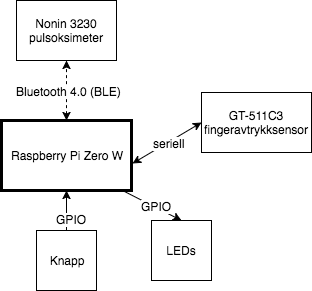
\includegraphics[width=0.55\textwidth, center]{fig/prototype/oversiktlosning}
\caption{Sammenhengen mellom de ulike komponentene}
\label{fig:prototypeoversikt}
\end{figure}

\section{Komponenter}

\subsection{Trykknapp og lysdioder}

\begin{figure}
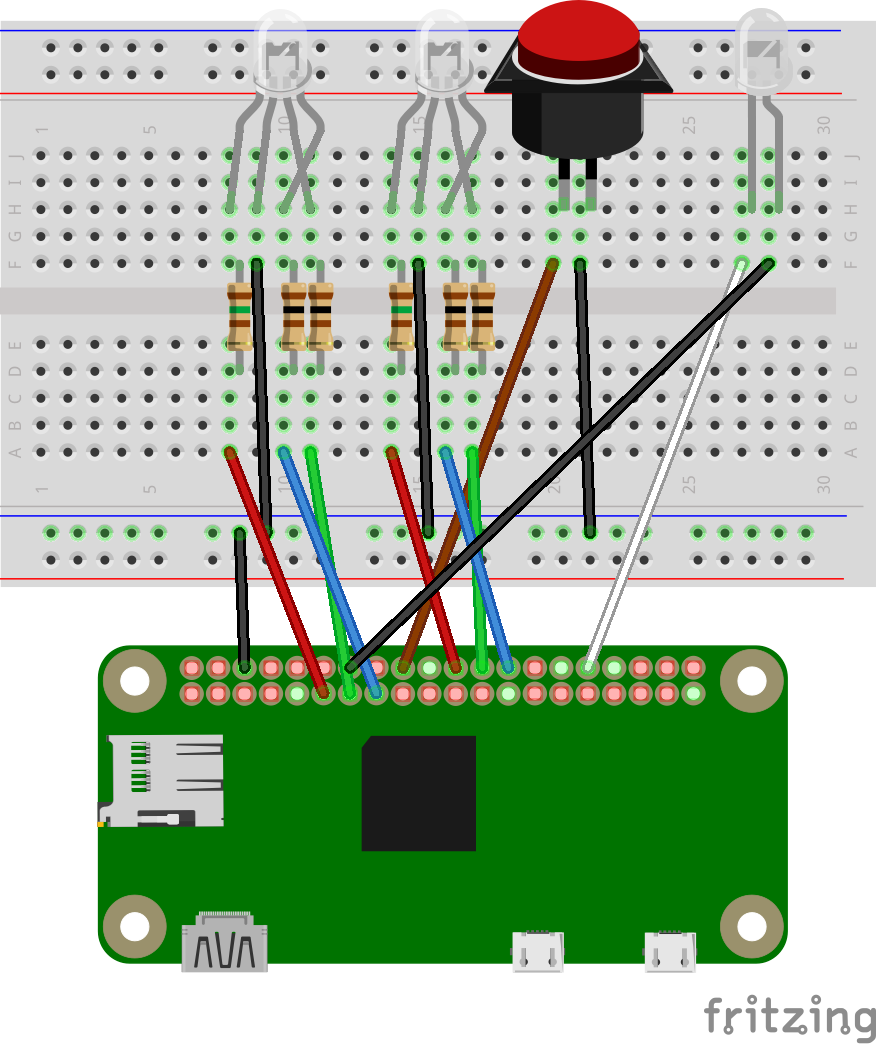
\includegraphics[width=0.75\textwidth, center]{fig/prototype/breadbord}
\caption{Oppkobling av trykkknapp og lysdioder}
\label{fig:breadboard}
\end{figure}

\begin{figure}
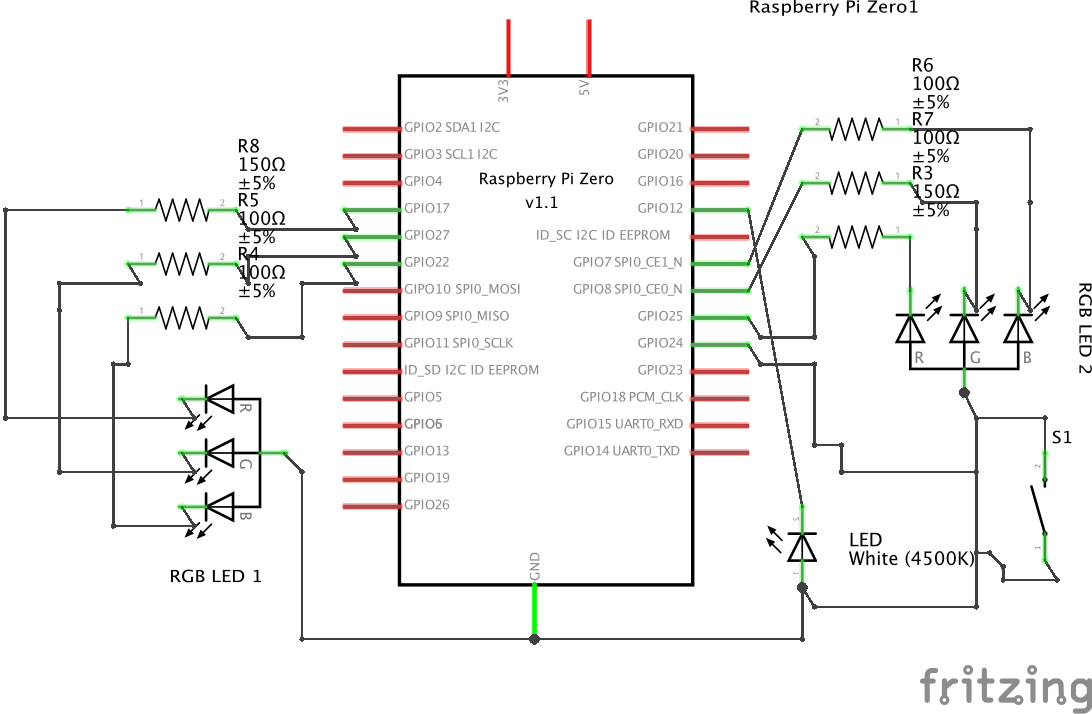
\includegraphics[width=0.95\textwidth, center]{fig/prototype/schmeatic}
\caption{Koplingsskjema av trykknapp og lysdioder}
\label{fig:schematics}
\end{figure}

\subsection{GT-511C3}

\subsection{Nonin 3230}
Trondheim kommune lånte ut en Nonin 3230 (se figur \ref{fig:nonin-3230}) til bruk i denne masteroppgaven.
Nonin 3230 er et pulsoksimeter med støtte for \gls{ble} 4.0. Dette pulsoksimeteret ble anbefalt av \citet{austad2016sensorer}
i rapporten «Sensorer til støtte for avstandsoppfølging». De trakk fram at alle Nonins produkter
er klinisk validerte, støtten for Bluetooth Smart,   

Utgaven Trondheim kommune har kjøpt inn bruker en proprietær Bluetooth-tjeneste med 128 bit \gls{uuid}.
I nyere utgaver kan man også bruke den åpne spesifikasjonen til «Bluetooth SIG Pulse Oximeter Service».
Den proprietære tjenesten heter «Nonin Oximetry Service» og har \gls{uuid} \textit{46a970e00d5f11e28b5e0002a5d5c51b}.
Tjenesten har to karakteristikker -- «Nonin Oximetry Measurement» som sender data hvert sekund som spesifiert
i tabell \ref{table:nonin-datapacket} og «Nonin Control Point» som kan brukes til å synkronisere skjermen,
indikere at en måling er ferdig, eller sette sikkerhetsmodus. 

Et \gls{npm}-biblotek (fotnote url) kalt \textit{nonin-3230-ble} ble utviklet for å gjøre integrasjonen mot sensoren enklere.
Biblioteket baserer seg på \textit{noble-device} (fotnote), og inneholder metoder for å oppdage et pulsoksimeter,
koble til, lytte etter ny sensordata og indikere at en måling er ferdig. Sensordata kommer som et JavaScript-objekt
og inneholder teller, pulsfrekvens, SpO2 og et statusobjekt (tabell \ref{table:nonin-status}).
Koden er lagt ved i appendiks \ref{lst:nonin-3230-library}.
Eksempel på bruk kan finnes i kodesnutt \ref{lst:nonin-3230-usage}.

\begin{figure}
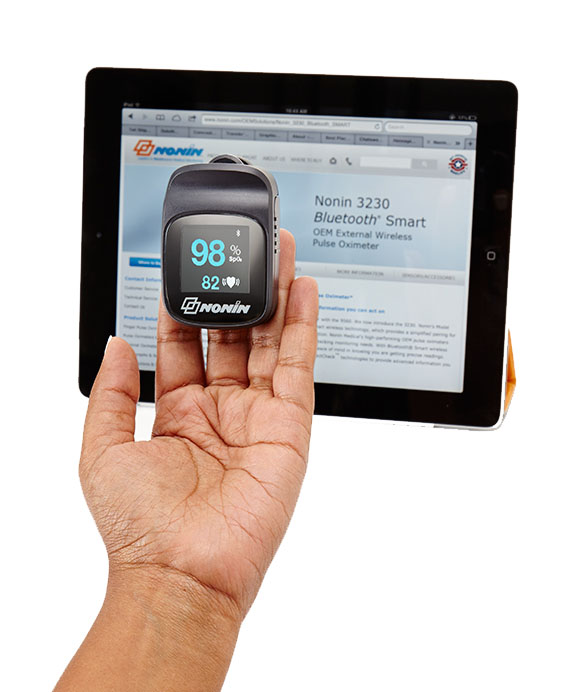
\includegraphics[width=0.95\textwidth, center]{fig/Nonin3230iPad}
\caption{Nonin 3230. Foto: Nonin}
\label{fig:nonin-3230}
\end{figure}

\begin{minipage}{\linewidth}
\begin{lstlisting}[frame=single, language=JavaScript,
    caption=Bruk av nonin-3230-ble, label=lst:nonin-3230-usage]
const Nonin3230 = require('nonin-3230-ble');

Nonin3230.discover((pulseOximeter) => {
  pulseOximeter.connectAndSetup((error) => {
    if (error) {
      console.error(error);
    }
    let counter = 0;
    // receive a new measurement every second
    pulseOximeter.on('data', (data) => {
      // data: { counter: int, pulseRate: int, oxygenSaturation: int, status: object }
      counter++;
      if (counter > 15) {
        pulseOximeter.stopMeasurement(() => console.log('Stopped'));
      }
    });
  });
});
\end{lstlisting}
\end{minipage}

Kildekoden er åpen og kan kjøres fra alle enheter som har støtte for Node og \gls{ble}.


\begin{table}[]
\centering
\begin{tabular}{|l|l|l}
\hline
\multicolumn{3}{|l|}{\textbf{Datapakke til oksimeter}} \\ \hline
\textbf{Byte} & \textbf{Felt} & \multicolumn{1}{l|}{\textbf{Beskrivelse}} \\ \hline
1 & Lengde & Antallet bytes inkludert denne. \\ \hline
2 & Status & \multicolumn{1}{l|}{Indikerer nåværende enhetsstatus (tabell \ref{table:nonin-status}).} \\ \hline
3 & Batterispenning & \multicolumn{1}{l|}{Spenningsnivået til batteriene som brukes.} \\ \hline
4-5 & \begin{tabular}[c]{@{}l@{}}Perfusjonsindeks\\ (PI)\end{tabular} & \multicolumn{1}{l|}{PI = AC/DC*100\%} \\ \hline
6-7 & Teller & \multicolumn{1}{l|}{\begin{tabular}[c]{@{}l@{}}Verdien økes hvert sekund (0-65535). Kan bli brukt\\ til å sjekke at det ikke er noe datatap.\end{tabular}} \\ \hline
8 & SpO2 & \multicolumn{1}{l|}{SpO2-prosent, 0-100 (gjennomsnitt av fire slag).} \\ \hline
9-10 & Pulsfrekvens & \multicolumn{1}{l|}{\begin{tabular}[c]{@{}l@{}}Pulsfrekvens i slag per minutt, 0-321\\ (gjennomsnitt av fire slag).\end{tabular}} \\ \hline
\textgreater11 & Reservert & \multicolumn{1}{l|}{Reservert til fremtidig bruk} \\ \hline
\end{tabular}
\caption{Nonin 3230: Format på datapakke ref: nonin integration guide}
\label{table:nonin-datapacket}
\end{table}

\begin{table}[]
\centering
\begin{tabular}{|l|l|l}
\hline
\multicolumn{3}{|l|}{\textbf{Statusfelt (aktiv høy)}} \\ \hline
\textbf{Bit} & \textbf{Felt} & \multicolumn{1}{l|}{\textbf{Beskrivelse}} \\ \hline
7 & Reservert & Reservert til fremtidig bruk. \\ \hline
6 & Kryptering & \multicolumn{1}{l|}{\begin{tabular}[c]{@{}l@{}}1 = tilkoblingen er kryptert\\ 2 = tilkoblingen er ikke kryptert\end{tabular}} \\ \hline
5 & Lavt batteri & \multicolumn{1}{l|}{Batterinivået er lavt. Bytt batteri.} \\ \hline
4 & CorrectCheck & \multicolumn{1}{l|}{\begin{tabular}[c]{@{}l@{}}1 = OK\\ 2 = Plasser fingeren lengre inn i enheten\end{tabular}} \\ \hline
3 & Søker & \multicolumn{1}{l|}{Oksimeteret søker etter etterfølgende pulssignaler.} \\ \hline
2 & SmartPoint & \multicolumn{1}{l|}{\begin{tabular}[c]{@{}l@{}}Brukt til å indikere at dataen har bestått SmartPoint-\\ algoritmen.\end{tabular}} \\ \hline
1 & Lavt/svakt signal & \multicolumn{1}{l|}{\begin{tabular}[c]{@{}l@{}}Styrken til pulssignalet er 0,3 \% modulasjonsgrad\\ eller mindre.\end{tabular}} \\ \hline
0 & \begin{tabular}[c]{@{}l@{}}Indikering av\\ skjermsynkronisering\end{tabular} & \multicolumn{1}{l|}{\begin{tabular}[c]{@{}l@{}}Indikerer at skjermen er synkronisert med\\ innsamleren av data.\end{tabular}} \\ \hline
\end{tabular}
\caption{Nonin 3230: Format på statusfeltet til datapakke ref: nonin integration guide}
\label{table:nonin-status}
\end{table}


\section{Serversideløsning}
\subsection{AWS IoT}
\subsection{AWS Lambda}
\subsection{InfluxDB og Grafana}

\subsection{Begrensninger med løsningen}